% Options for packages loaded elsewhere
% Options for packages loaded elsewhere
\PassOptionsToPackage{unicode}{hyperref}
\PassOptionsToPackage{hyphens}{url}
\PassOptionsToPackage{dvipsnames,svgnames,x11names}{xcolor}
%
\documentclass[
  letterpaper,
  DIV=11,
  numbers=noendperiod]{scrartcl}
\usepackage{xcolor}
\usepackage{amsmath,amssymb}
\setcounter{secnumdepth}{5}
\usepackage{iftex}
\ifPDFTeX
  \usepackage[T1]{fontenc}
  \usepackage[utf8]{inputenc}
  \usepackage{textcomp} % provide euro and other symbols
\else % if luatex or xetex
  \usepackage{unicode-math} % this also loads fontspec
  \defaultfontfeatures{Scale=MatchLowercase}
  \defaultfontfeatures[\rmfamily]{Ligatures=TeX,Scale=1}
\fi
\usepackage{lmodern}
\ifPDFTeX\else
  % xetex/luatex font selection
\fi
% Use upquote if available, for straight quotes in verbatim environments
\IfFileExists{upquote.sty}{\usepackage{upquote}}{}
\IfFileExists{microtype.sty}{% use microtype if available
  \usepackage[]{microtype}
  \UseMicrotypeSet[protrusion]{basicmath} % disable protrusion for tt fonts
}{}
\makeatletter
\@ifundefined{KOMAClassName}{% if non-KOMA class
  \IfFileExists{parskip.sty}{%
    \usepackage{parskip}
  }{% else
    \setlength{\parindent}{0pt}
    \setlength{\parskip}{6pt plus 2pt minus 1pt}}
}{% if KOMA class
  \KOMAoptions{parskip=half}}
\makeatother

\usepackage{color}
\usepackage{fancyvrb}
\newcommand{\VerbBar}{|}
\newcommand{\VERB}{\Verb[commandchars=\\\{\}]}
\DefineVerbatimEnvironment{Highlighting}{Verbatim}{commandchars=\\\{\}}
% Add ',fontsize=\small' for more characters per line
\usepackage{framed}
\definecolor{shadecolor}{RGB}{241,243,245}
\newenvironment{Shaded}{\begin{snugshade}}{\end{snugshade}}
\newcommand{\AlertTok}[1]{\textcolor[rgb]{0.68,0.00,0.00}{#1}}
\newcommand{\AnnotationTok}[1]{\textcolor[rgb]{0.37,0.37,0.37}{#1}}
\newcommand{\AttributeTok}[1]{\textcolor[rgb]{0.40,0.45,0.13}{#1}}
\newcommand{\BaseNTok}[1]{\textcolor[rgb]{0.68,0.00,0.00}{#1}}
\newcommand{\BuiltInTok}[1]{\textcolor[rgb]{0.00,0.23,0.31}{#1}}
\newcommand{\CharTok}[1]{\textcolor[rgb]{0.13,0.47,0.30}{#1}}
\newcommand{\CommentTok}[1]{\textcolor[rgb]{0.37,0.37,0.37}{#1}}
\newcommand{\CommentVarTok}[1]{\textcolor[rgb]{0.37,0.37,0.37}{\textit{#1}}}
\newcommand{\ConstantTok}[1]{\textcolor[rgb]{0.56,0.35,0.01}{#1}}
\newcommand{\ControlFlowTok}[1]{\textcolor[rgb]{0.00,0.23,0.31}{\textbf{#1}}}
\newcommand{\DataTypeTok}[1]{\textcolor[rgb]{0.68,0.00,0.00}{#1}}
\newcommand{\DecValTok}[1]{\textcolor[rgb]{0.68,0.00,0.00}{#1}}
\newcommand{\DocumentationTok}[1]{\textcolor[rgb]{0.37,0.37,0.37}{\textit{#1}}}
\newcommand{\ErrorTok}[1]{\textcolor[rgb]{0.68,0.00,0.00}{#1}}
\newcommand{\ExtensionTok}[1]{\textcolor[rgb]{0.00,0.23,0.31}{#1}}
\newcommand{\FloatTok}[1]{\textcolor[rgb]{0.68,0.00,0.00}{#1}}
\newcommand{\FunctionTok}[1]{\textcolor[rgb]{0.28,0.35,0.67}{#1}}
\newcommand{\ImportTok}[1]{\textcolor[rgb]{0.00,0.46,0.62}{#1}}
\newcommand{\InformationTok}[1]{\textcolor[rgb]{0.37,0.37,0.37}{#1}}
\newcommand{\KeywordTok}[1]{\textcolor[rgb]{0.00,0.23,0.31}{\textbf{#1}}}
\newcommand{\NormalTok}[1]{\textcolor[rgb]{0.00,0.23,0.31}{#1}}
\newcommand{\OperatorTok}[1]{\textcolor[rgb]{0.37,0.37,0.37}{#1}}
\newcommand{\OtherTok}[1]{\textcolor[rgb]{0.00,0.23,0.31}{#1}}
\newcommand{\PreprocessorTok}[1]{\textcolor[rgb]{0.68,0.00,0.00}{#1}}
\newcommand{\RegionMarkerTok}[1]{\textcolor[rgb]{0.00,0.23,0.31}{#1}}
\newcommand{\SpecialCharTok}[1]{\textcolor[rgb]{0.37,0.37,0.37}{#1}}
\newcommand{\SpecialStringTok}[1]{\textcolor[rgb]{0.13,0.47,0.30}{#1}}
\newcommand{\StringTok}[1]{\textcolor[rgb]{0.13,0.47,0.30}{#1}}
\newcommand{\VariableTok}[1]{\textcolor[rgb]{0.07,0.07,0.07}{#1}}
\newcommand{\VerbatimStringTok}[1]{\textcolor[rgb]{0.13,0.47,0.30}{#1}}
\newcommand{\WarningTok}[1]{\textcolor[rgb]{0.37,0.37,0.37}{\textit{#1}}}

\usepackage{longtable,booktabs,array}
\usepackage{calc} % for calculating minipage widths
\usepackage{caption}
% Make caption package work with longtable
\makeatletter
\def\fnum@table{\tablename~\thetable}
\makeatother
\usepackage{graphicx}
\makeatletter
\newsavebox\pandoc@box
\newcommand*\pandocbounded[1]{% scales image to fit in text height/width
  \sbox\pandoc@box{#1}%
  \Gscale@div\@tempa{\textheight}{\dimexpr\ht\pandoc@box+\dp\pandoc@box\relax}%
  \Gscale@div\@tempb{\linewidth}{\wd\pandoc@box}%
  \ifdim\@tempb\p@<\@tempa\p@\let\@tempa\@tempb\fi% select the smaller of both
  \ifdim\@tempa\p@<\p@\scalebox{\@tempa}{\usebox\pandoc@box}%
  \else\usebox{\pandoc@box}%
  \fi%
}
% Set default figure placement to htbp
\def\fps@figure{htbp}
\makeatother


% definitions for citeproc citations
\NewDocumentCommand\citeproctext{}{}
\NewDocumentCommand\citeproc{mm}{%
  \begingroup\def\citeproctext{#2}\cite{#1}\endgroup}
\makeatletter
 % allow citations to break across lines
 \let\@cite@ofmt\@firstofone
 % avoid brackets around text for \cite:
 \def\@biblabel#1{}
 \def\@cite#1#2{{#1\if@tempswa , #2\fi}}
\makeatother
\newlength{\cslhangindent}
\setlength{\cslhangindent}{1.5em}
\newlength{\csllabelwidth}
\setlength{\csllabelwidth}{3em}
\newenvironment{CSLReferences}[2] % #1 hanging-indent, #2 entry-spacing
 {\begin{list}{}{%
  \setlength{\itemindent}{0pt}
  \setlength{\leftmargin}{0pt}
  \setlength{\parsep}{0pt}
  % turn on hanging indent if param 1 is 1
  \ifodd #1
   \setlength{\leftmargin}{\cslhangindent}
   \setlength{\itemindent}{-1\cslhangindent}
  \fi
  % set entry spacing
  \setlength{\itemsep}{#2\baselineskip}}}
 {\end{list}}
\usepackage{calc}
\newcommand{\CSLBlock}[1]{\hfill\break\parbox[t]{\linewidth}{\strut\ignorespaces#1\strut}}
\newcommand{\CSLLeftMargin}[1]{\parbox[t]{\csllabelwidth}{\strut#1\strut}}
\newcommand{\CSLRightInline}[1]{\parbox[t]{\linewidth - \csllabelwidth}{\strut#1\strut}}
\newcommand{\CSLIndent}[1]{\hspace{\cslhangindent}#1}



\setlength{\emergencystretch}{3em} % prevent overfull lines

\providecommand{\tightlist}{%
  \setlength{\itemsep}{0pt}\setlength{\parskip}{0pt}}



 


\KOMAoption{captions}{tableheading}
\makeatletter
\@ifpackageloaded{caption}{}{\usepackage{caption}}
\AtBeginDocument{%
\ifdefined\contentsname
  \renewcommand*\contentsname{Table of contents}
\else
  \newcommand\contentsname{Table of contents}
\fi
\ifdefined\listfigurename
  \renewcommand*\listfigurename{List of Figures}
\else
  \newcommand\listfigurename{List of Figures}
\fi
\ifdefined\listtablename
  \renewcommand*\listtablename{List of Tables}
\else
  \newcommand\listtablename{List of Tables}
\fi
\ifdefined\figurename
  \renewcommand*\figurename{Figure}
\else
  \newcommand\figurename{Figure}
\fi
\ifdefined\tablename
  \renewcommand*\tablename{Table}
\else
  \newcommand\tablename{Table}
\fi
}
\@ifpackageloaded{float}{}{\usepackage{float}}
\floatstyle{ruled}
\@ifundefined{c@chapter}{\newfloat{codelisting}{h}{lop}}{\newfloat{codelisting}{h}{lop}[chapter]}
\floatname{codelisting}{Listing}
\newcommand*\listoflistings{\listof{codelisting}{List of Listings}}
\makeatother
\makeatletter
\makeatother
\makeatletter
\@ifpackageloaded{caption}{}{\usepackage{caption}}
\@ifpackageloaded{subcaption}{}{\usepackage{subcaption}}
\makeatother
\usepackage{bookmark}
\IfFileExists{xurl.sty}{\usepackage{xurl}}{} % add URL line breaks if available
\urlstyle{same}
\hypersetup{
  pdftitle={Análisis de Supervivencia},
  pdfauthor={Sergio M. Nava Muñoz},
  colorlinks=true,
  linkcolor={blue},
  filecolor={Maroon},
  citecolor={Blue},
  urlcolor={Blue},
  pdfcreator={LaTeX via pandoc}}


\title{Análisis de Supervivencia}
\usepackage{etoolbox}
\makeatletter
\providecommand{\subtitle}[1]{% add subtitle to \maketitle
  \apptocmd{\@title}{\par {\large #1 \par}}{}{}
}
\makeatother
\subtitle{Funciones fundamentales de Análisis de Supervivencia}
\author{Sergio M. Nava Muñoz}
\date{2025-06-01}
\begin{document}
\maketitle


\section{Funciones fundamentales de Análisis de
Supervivencia}\label{funciones-fundamentales-de-anuxe1lisis-de-supervivencia}

\subsection{Introducción}\label{introducciuxf3n}

En esta sección abordaremos los conceptos fundamentales para el análisis
de datos de supervivencia, comenzando con funciones de probabilidad
clásicas y avanzando hacia funciones específicas como la función de
supervivencia y la función de riesgo.

\subsubsection{Objetivos}\label{objetivos}

\begin{itemize}
\tightlist
\item
  Recordar las funciones de densidad y distribución acumulada.
\item
  Introducir la función de supervivencia \(S(t)\) y la función de riesgo
  \(h(t)\).
\item
  Interpretar estas funciones desde una perspectiva probabilística.
\item
  Visualizar ejemplos aplicados y comparativos con distintas
  distribuciones.
\end{itemize}

\subsection{Funciones fundamentales}\label{funciones-fundamentales}

Antes de introducir las funciones de supervivencia y riesgo, recordemos
dos funciones clave en probabilidad y estadística:

\begin{itemize}
\tightlist
\item
  \textbf{Función de densidad}: \(f(t)\)
\item
  \textbf{Función de distribución acumulada}: \(F(t) = P(T \leq t)\)
\end{itemize}

\begin{center}\rule{0.5\linewidth}{0.5pt}\end{center}

\subsubsection{\texorpdfstring{Función de densidad
\(f(t)\)}{Función de densidad f(t)}}\label{funciuxf3n-de-densidad-ft}

\begin{itemize}
\item
  Describe la distribución de probabilidad de una variable continua
  \(T\)
\item
  No es una probabilidad en sí, pero su integral sí lo es:

  \[
  P(a < T \leq b) = \int_a^b f(t) \, dt
  \]
\item
  Debe cumplir:

  \[
  f(t) \geq 0 \quad \text{y} \quad \int_{-\infty}^{\infty} f(t) \, dt = 1
  \]
\end{itemize}

\begin{center}\rule{0.5\linewidth}{0.5pt}\end{center}

\subsubsection{\texorpdfstring{Función de distribución acumulada
\(F(t)\)}{Función de distribución acumulada F(t)}}\label{funciuxf3n-de-distribuciuxf3n-acumulada-ft}

\begin{itemize}
\item
  Es la probabilidad de que la variable aleatoria tome un valor menor o
  igual que \(t\):

  \[
  F(t) = \int_{-\infty}^t f(u) \, du = P(T \leq t)
  \]
\item
  Propiedades:

  \begin{itemize}
  \tightlist
  \item
    \(F(t)\) es monótona creciente
  \item
    \(\lim_{t \to -\infty} F(t) = 0\)
  \item
    \(\lim_{t \to \infty} F(t) = 1\)
  \end{itemize}
\end{itemize}

\begin{center}\rule{0.5\linewidth}{0.5pt}\end{center}

\subsubsection{\texorpdfstring{Relación entre \(f(t)\) y
\(F(t)\)}{Relación entre f(t) y F(t)}}\label{relaciuxf3n-entre-ft-y-ft}

\begin{itemize}
\item
  Si \(f\) es continua:

  \[
  f(t) = \frac{d}{dt} F(t)
  \]
\item
  Y también:

  \[
  F(t) = \int_{-\infty}^t f(u) \, du
  \]
\end{itemize}

Estas relaciones son clave para definir funciones como la de
supervivencia y la de riesgo, que veremos a continuación.

\subsubsection{\texorpdfstring{Ejemplo en R: distribución distribución
exponencial con parámetro
\(\lambda = 0.5\)}{Ejemplo en R: distribución distribución exponencial con parámetro \textbackslash lambda = 0.5}}\label{ejemplo-en-r-distribuciuxf3n-distribuciuxf3n-exponencial-con-paruxe1metro-lambda-0.5}

\pandocbounded{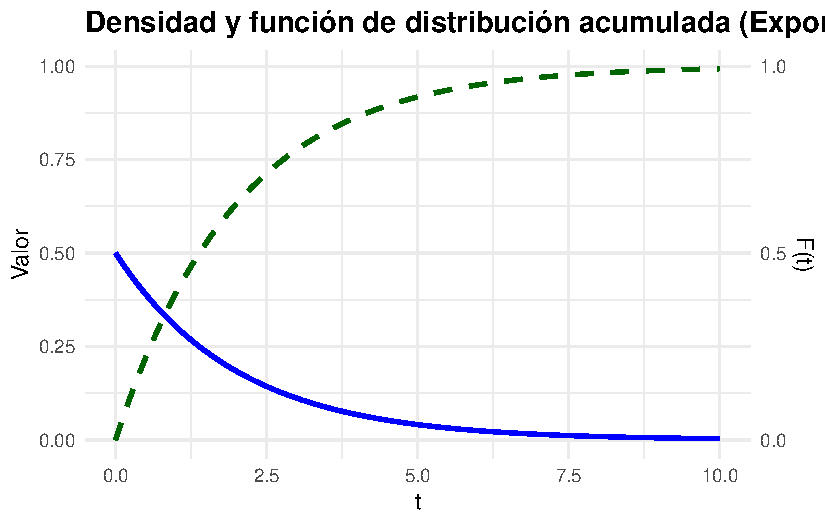
\includegraphics[keepaspectratio]{Unidad2_files/figure-pdf/unnamed-chunk-2-1.pdf}}

\subsection{Funciones fundamentales en análisis de
supervivencia}\label{funciones-fundamentales-en-anuxe1lisis-de-supervivencia}

\begin{quote}
En análisis de supervivencia, las variables aleatorias de interés \(T\)
son no negativas, y se caracterizan no solo por \(f(t)\) o \(F(t)\),
sino también por funciones \textbf{más interpretables}:
\end{quote}

\begin{itemize}
\tightlist
\item
  \(S(t)\): función de supervivencia
\item
  \(h(t)\): función de riesgo o tasa de falla
\item
  \(H(t)\): riesgo acumulado
\end{itemize}

\section{\texorpdfstring{Función de supervivencia
\(S(t)\)}{Función de supervivencia S(t)}}\label{funciuxf3n-de-supervivencia-st}

\subsection{Función de Supervivencia}\label{funciuxf3n-de-supervivencia}

La función de supervivencia \(S(t)\) y la función de riesgo instantáneo
\(h(t)\) son fundamentales para modelar procesos de falla en este tipo
de análisis, ver Klein \& Moeschberger (2003).

\begin{quote}
\(S(t) = P(T > t) = 1 - F(t)\)
\end{quote}

Representa la probabilidad de \textbf{sobrevivir más allá del tiempo}
\(t\).

\textbf{Propiedades clave}:

\begin{itemize}
\tightlist
\item
  Monótona no creciente\\
\item
  \(S(0) = 1\), \(\lim_{t \to \infty} S(t) = 0\)
\end{itemize}

\begin{center}
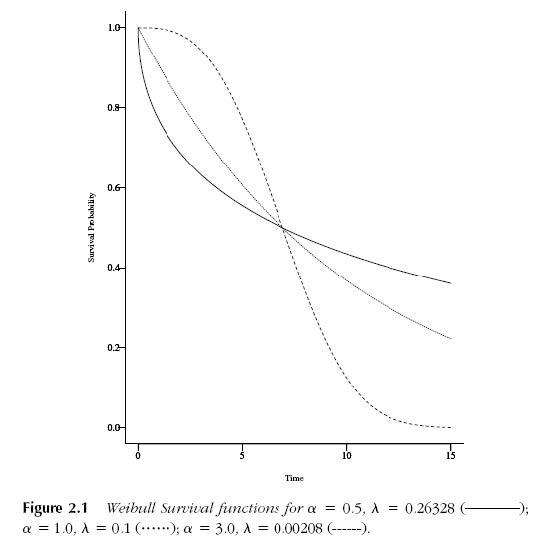
\includegraphics[width=0.7\linewidth,height=\textheight,keepaspectratio]{figura/Ss.jpg}
\end{center}

\begin{center}\rule{0.5\linewidth}{0.5pt}\end{center}

\subsection{Ejemplo: función de supervivencia para distribución
exponencial}\label{ejemplo-funciuxf3n-de-supervivencia-para-distribuciuxf3n-exponencial}

Sea \(T \sim \text{Exp}(\lambda = 0.5)\), es decir:

\[
f(t) = \lambda e^{-\lambda t}, \quad F(t)=1-e^{-\lambda t}, \quad S(t) = e^{-\lambda t}
\]

\pandocbounded{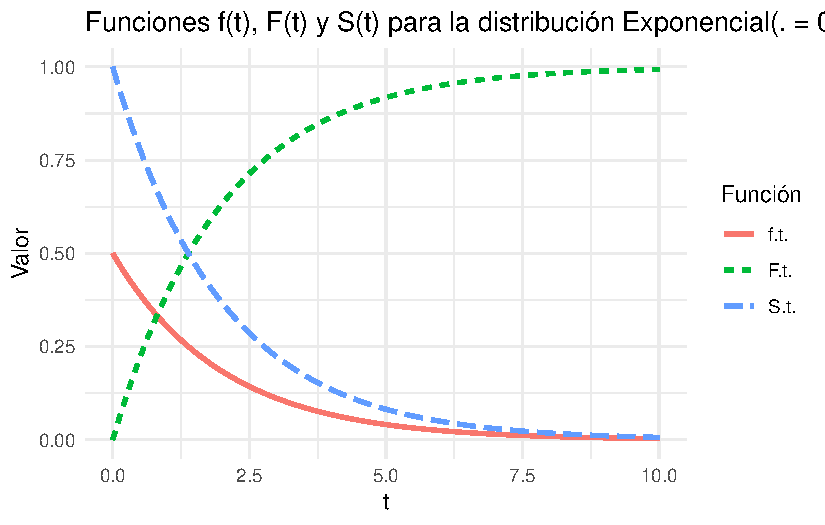
\includegraphics[keepaspectratio]{Unidad2_files/figure-pdf/unnamed-chunk-3-1.pdf}}

\section{\texorpdfstring{Función de riesgo
\(h(t)\)}{Función de riesgo h(t)}}\label{funciuxf3n-de-riesgo-ht}

\subsection{Función de Riesgo}\label{funciuxf3n-de-riesgo}

\begin{quote}
\(h(t) = \frac{f(t)}{S(t)}\)
\end{quote}

\begin{itemize}
\tightlist
\item
  También conocida como:

  \begin{itemize}
  \tightlist
  \item
    Tasa de falla condicional (confiabilidad)
  \item
    Tasa de mortalidad (demografía)
  \item
    Función de intensidad (procesos estocásticos)
  \end{itemize}
\end{itemize}

\textbf{Interpretación}:\\
Tasa instantánea de ocurrencia del evento, dado que se ha sobrevivido
hasta \(t\).

\begin{center}\rule{0.5\linewidth}{0.5pt}\end{center}

\subsection{Ejemplos de formas de
riesgo}\label{ejemplos-de-formas-de-riesgo}

\begin{longtable}[]{@{}ll@{}}
\toprule\noalign{}
Forma del riesgo & Interpretación \\
\midrule\noalign{}
\endhead
\bottomrule\noalign{}
\endlastfoot
Riesgo creciente & Envejecimiento \\
Riesgo decreciente & Rejuvenecimiento \\
Riesgo tipo ``tina de baño'' & Mortalidad neonatal y senil \\
Riesgo tipo ``montaña'' & Recaída tras tratamiento \\
\end{longtable}

\pandocbounded{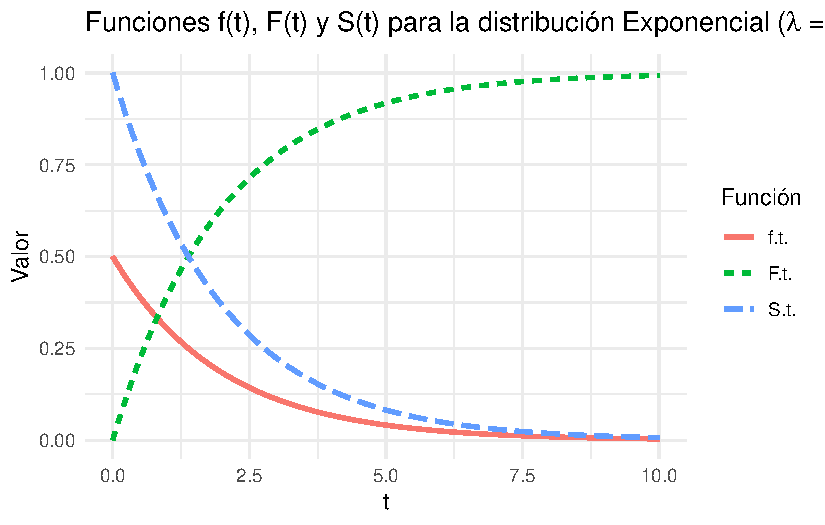
\includegraphics[keepaspectratio]{Unidad2_files/figure-pdf/unnamed-chunk-4-1.pdf}}

\subsection{Ejemplo: función de riesgo para distribuciones
comunes}\label{ejemplo-funciuxf3n-de-riesgo-para-distribuciones-comunes}

\[
h(t) = \frac{f(t)}{S(t)}
\]

Para la distribución exponencial con \(\lambda = 0.5\),
\(h(t) = \lambda\), constante.

Comparémosla con la distribución Weibull, donde el riesgo puede aumentar
o disminuir con el tiempo.

\pandocbounded{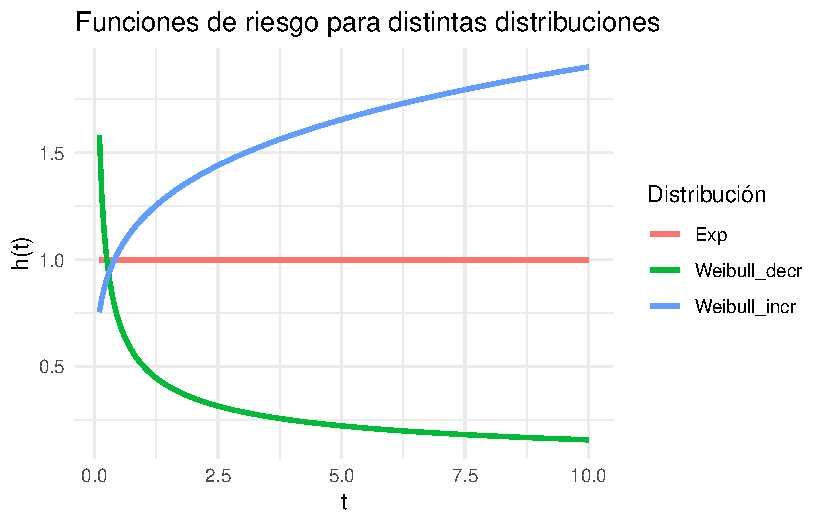
\includegraphics[keepaspectratio]{Unidad2_files/figure-pdf/unnamed-chunk-5-1.pdf}}

\begin{center}\rule{0.5\linewidth}{0.5pt}\end{center}

\subsection{Otra forma de
visualización}\label{otra-forma-de-visualizaciuxf3n}

\begin{center}
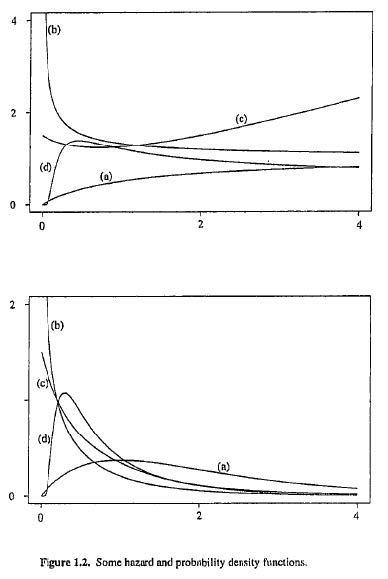
\includegraphics[width=4in,height=\textheight,keepaspectratio]{figura/ejempRiesgoContinuo2.jpg}
\end{center}

\section{Tiempo discreto}\label{tiempo-discreto}

\subsection{Riesgo en tiempo discreto}\label{riesgo-en-tiempo-discreto}

Para \(T\) discreta con soporte \(\{u_1, u_2, \dots\}\):

\[
h(t) = P(T = t \mid T \ge t)
\]

\[
h_k = \frac{P(T = u_k)}{P(T \ge u_k)} = \frac{f(u_k)}{S(u_{k-1})}
\]

Usando \(f(u_k) = S(u_{k-1}) - S(u_k)\), se obtiene:

\[
h_k = 1 - \frac{S(u_k)}{S(u_{k-1})}
\]

\begin{center}\rule{0.5\linewidth}{0.5pt}\end{center}

\subsection{Relaciones discretas
clave}\label{relaciones-discretas-clave}

Función de supervivencia:

\[
S(t) = \prod_{u_k \le t} (1 - h_k)
\]

Función de densidad:

\[
f(u_j) = h_j \prod_{k<j} (1 - h_k)
\]

\begin{quote}
En demografía, \(h(t)\) representa la probabilidad de morir en el
momento \(t\) dado que se ha sobrevivido hasta \(t\).
\end{quote}

\begin{center}\rule{0.5\linewidth}{0.5pt}\end{center}

\subsection{Ejemplos de riesgo
discreto}\label{ejemplos-de-riesgo-discreto}

\begin{center}
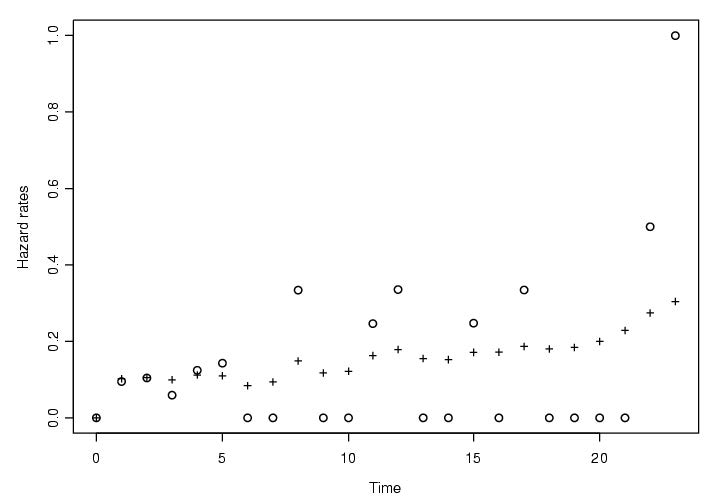
\includegraphics[width=4in,height=\textheight,keepaspectratio]{figura/ejempRiesgoDiscreto.jpg}
\end{center}

\begin{center}\rule{0.5\linewidth}{0.5pt}\end{center}

\subsection{Riesgo acumulado discreto}\label{riesgo-acumulado-discreto}

Dos definiciones equivalentes:

\begin{enumerate}
\def\labelenumi{\arabic{enumi}.}
\item
  Suma directa: \[
  H(t) = \sum_{u_k \le t} h_k
  \]
\item
  Log-transformación: \[
  H(t) = - \sum_{u_k \le t} \log(1 - h_k)
  \]
\end{enumerate}

Ambas son \textbf{monótonas no decrecientes}.

\section{Tiempo contínuo}\label{tiempo-contuxednuo}

\subsection{Riesgo en tiempo continuo}\label{riesgo-en-tiempo-continuo}

\[
h(t) = \lim_{\varepsilon \to 0} \frac{1}{\varepsilon} P(t < T \le t + \varepsilon \mid T \ge t)
= \frac{f(t)}{S(t)}
\]

Como \(F(t) = 1 - S(t)\), entonces:

\[
h(t) = -\frac{d}{dt} \log S(t)
\]

Al integrar:

\[
\log S(t) = -\int_0^t h(u) \, du
\]

\[
S(t) = \exp\left(-\int_0^t h(u) \, du\right)
\]

\begin{quote}
\(h(t)\varepsilon\) es la probabilidad \textbf{aproximada} de que un
evento ocurra en el siguiente instante dado que el individuo ha
sobrevivido hasta \(t\).
\end{quote}

\begin{center}\rule{0.5\linewidth}{0.5pt}\end{center}

\subsection{Riesgo acumulado continuo}\label{riesgo-acumulado-continuo}

\[
H(t) = \int_0^t h(u)\, du
\qquad\Rightarrow\qquad
S(t) = \exp\{-H(t)\}
\]

Si \(S(\infty) = 0\), entonces \(H(\infty) = \infty\).

\begin{center}\rule{0.5\linewidth}{0.5pt}\end{center}

\subsection{Visualización de
funciones}\label{visualizaciuxf3n-de-funciones}

\begin{center}
\pandocbounded{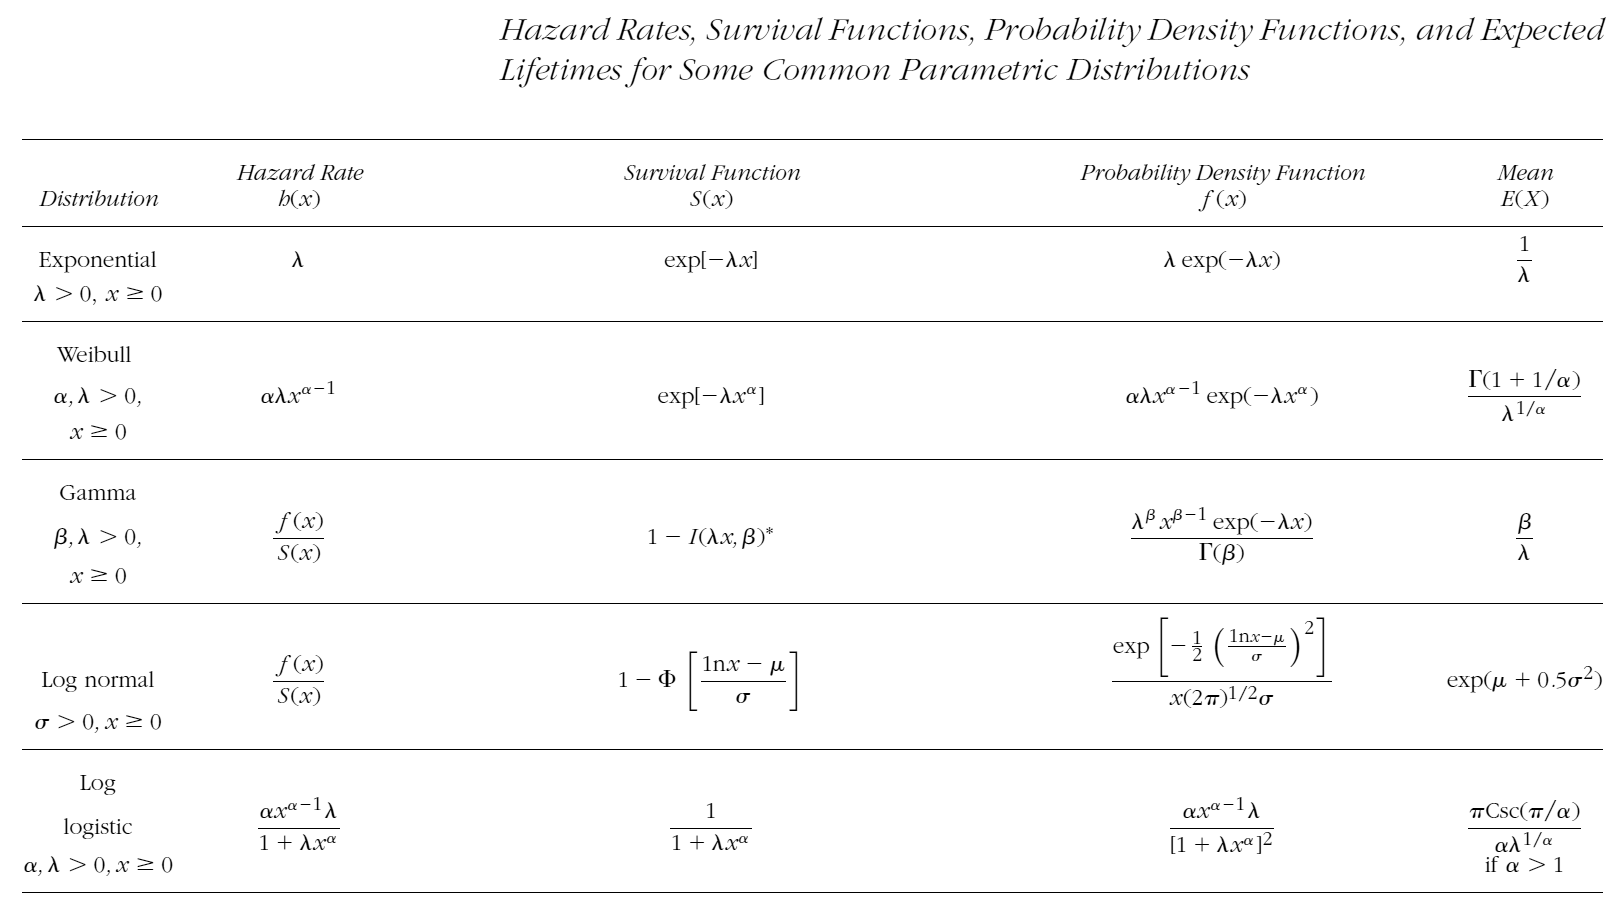
\includegraphics[keepaspectratio]{figura/Funciones1.png}}
\end{center}

\begin{center}\rule{0.5\linewidth}{0.5pt}\end{center}

\subsection{Visualización de funciones
(cont.)}\label{visualizaciuxf3n-de-funciones-cont.}

\begin{center}
\pandocbounded{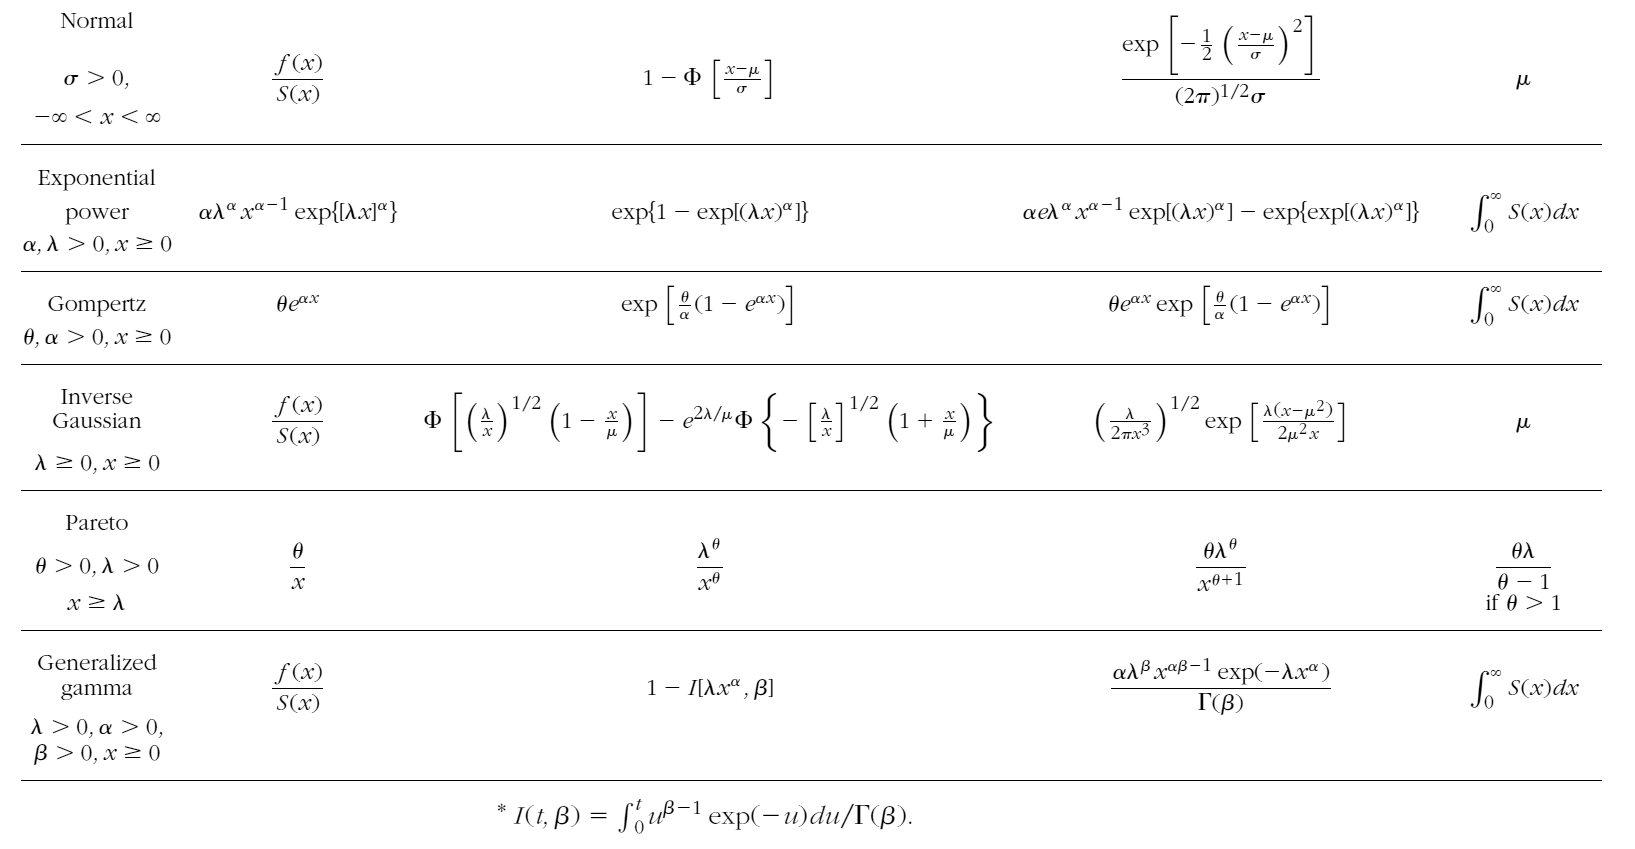
\includegraphics[keepaspectratio]{figura/Funciones2.png}}
\end{center}

\subsection{Visualización de Funciones en
R}\label{visualizaciuxf3n-de-funciones-en-r}

Las funciones \texttt{Surv()} y \texttt{survfit()} del paquete
\texttt{survival} permiten ajustar y visualizar curvas de Kaplan-Meier
de manera eficiente en R, ver Moore (2016) y Therneau \& Grambsch
(2000).

\begin{Shaded}
\begin{Highlighting}[]
\CommentTok{\# Ejemplo simulado de tiempos de supervivencia}
\FunctionTok{set.seed}\NormalTok{(}\DecValTok{123}\NormalTok{)}
\NormalTok{tiempos }\OtherTok{\textless{}{-}} \FunctionTok{rexp}\NormalTok{(}\DecValTok{10}\NormalTok{, }\AttributeTok{rate =} \FloatTok{0.05}\NormalTok{)}
\NormalTok{status }\OtherTok{\textless{}{-}} \FunctionTok{rbinom}\NormalTok{(}\DecValTok{10}\NormalTok{, }\DecValTok{1}\NormalTok{, }\AttributeTok{prob =} \FloatTok{0.8}\NormalTok{)}
\NormalTok{data\_sim }\OtherTok{\textless{}{-}} \FunctionTok{data.frame}\NormalTok{(}\AttributeTok{time =}\NormalTok{ tiempos, }\AttributeTok{event =}\NormalTok{ status)}
\CommentTok{\# Estimación Kaplan{-}Meier}
\NormalTok{km\_fit }\OtherTok{\textless{}{-}} \FunctionTok{survfit}\NormalTok{(}\FunctionTok{Surv}\NormalTok{(time, event) }\SpecialCharTok{\textasciitilde{}} \DecValTok{1}\NormalTok{, }\AttributeTok{data =}\NormalTok{ data\_sim)}
\end{Highlighting}
\end{Shaded}

\begin{longtable}[]{@{}rr@{}}
\caption{data\_sim}\tabularnewline
\toprule\noalign{}
time & event \\
\midrule\noalign{}
\endfirsthead
\toprule\noalign{}
time & event \\
\midrule\noalign{}
\endhead
\bottomrule\noalign{}
\endlastfoot
16.8691452 & 1 \\
11.5322054 & 0 \\
26.5810974 & 0 \\
0.6315472 & 1 \\
1.1242195 & 1 \\
6.3300243 & 0 \\
6.2845458 & 1 \\
2.9053361 & 1 \\
54.5247293 & 1 \\
0.5830689 & 1 \\
\end{longtable}

\begin{Shaded}
\begin{Highlighting}[]
\FunctionTok{plot}\NormalTok{(km\_fit, }
     \AttributeTok{xlab =} \StringTok{"Tiempo"}\NormalTok{, }
     \AttributeTok{ylab =} \StringTok{"Supervivencia"}\NormalTok{, }
     \AttributeTok{main =} \StringTok{"Curva Kaplan{-}Meier"}\NormalTok{)}
\end{Highlighting}
\end{Shaded}

\pandocbounded{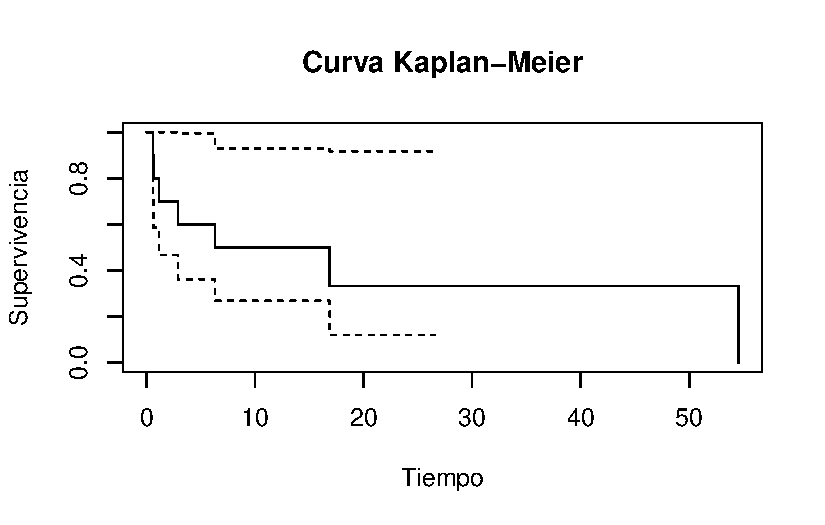
\includegraphics[keepaspectratio]{Unidad2_files/figure-pdf/unnamed-chunk-8-1.pdf}}

\section{Referencias}\label{referencias}

\phantomsection\label{refs}
\begin{CSLReferences}{1}{0}
\bibitem[\citeproctext]{ref-klein2003}
Klein, J. P., \& Moeschberger, M. L. (2003). \emph{Survival analysis:
Techniques for censored and truncated data} (2nd ed.). Springer.

\bibitem[\citeproctext]{ref-moore2016}
Moore, D. F. (2016). \emph{Applied survival analysis using r} (2nd ed.).
Springer. \url{https://doi.org/10.1007/978-3-319-31245-3}

\bibitem[\citeproctext]{ref-therneau2000}
Therneau, T. M., \& Grambsch, P. M. (2000). \emph{Modeling survival
data: Extending the cox model}. Springer.

\end{CSLReferences}




\end{document}
